\section{Requirement And Specification}


\subsection{Scope}

\begin{frame}{\currentname}

The \emph{myTaxiService} software focuses on helping the clients benefit from the service and ensures a fair management of taxi queues.

\vfill

\begin{columns}[c]
  \begin{column}{.5\textwidth}
    The software will:
    \begin{itemize}
    \item give the possibility to request a taxi either through a web application or a mobile app.
    \item compute the distribution of taxis in the various zones based on the GPS information it receives from each taxi.
    \item offer programmatic interfaces to enable the development of additional services.
    \item allow to book a taxi by specifying the origin and the destination of the ride.
    \end{itemize}
  \end{column}
  \begin{column}{.47\textwidth}
    
\includegraphics[width=\textwidth]{taxi-cab}
		\centering
  \end{column}
\end{columns}

\end{frame}

\subsection{User Interfaces}

\subsubsection{Clients' User Interfaces}
\begin{frame}{\currentname{}}
\begin{columns}[c]
  \begin{column}{.5\textwidth}
		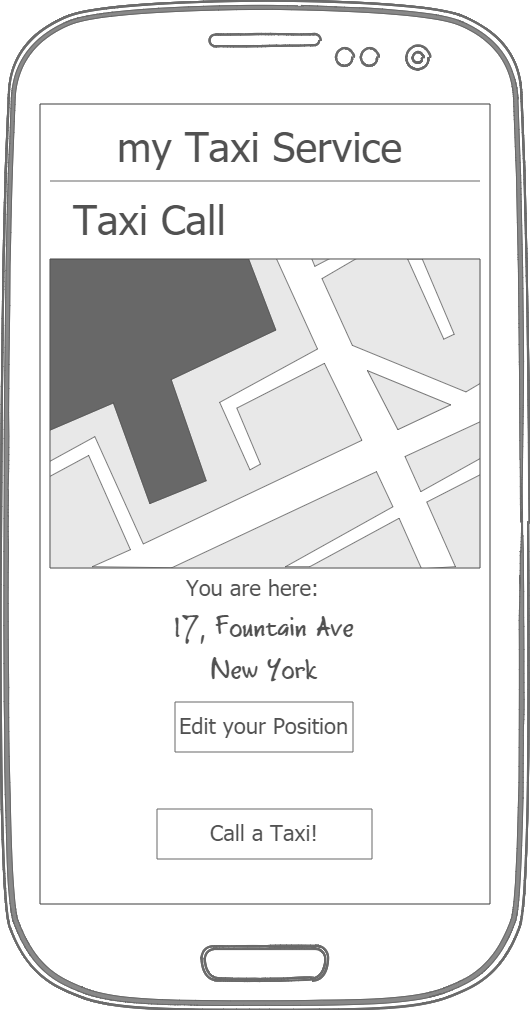
\includegraphics[height=.8\textheight]{Mockup-ClientsTaxiCall}
		\centering
  \end{column}
  \begin{column}{.5\textwidth}
    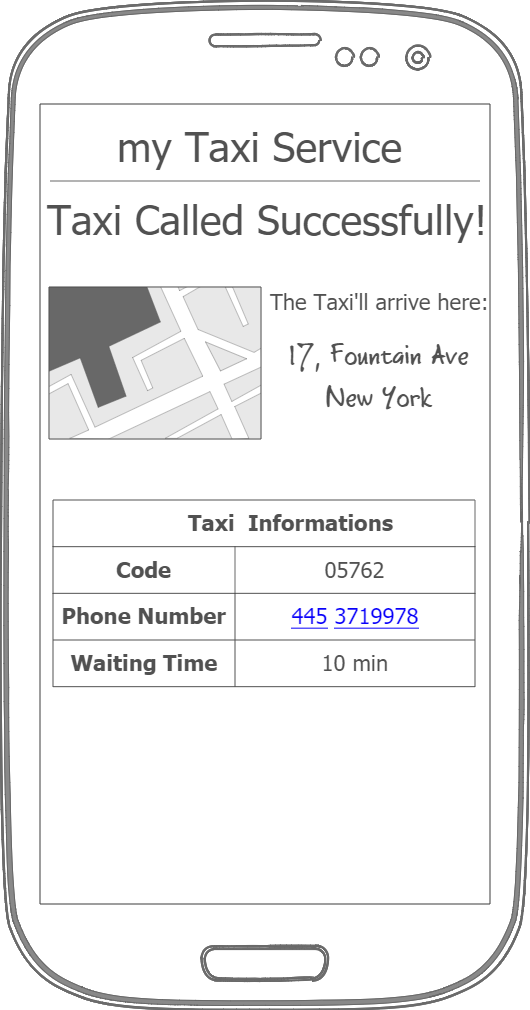
\includegraphics[height=.8\textheight]{Mockup-ClientsTaxiCallConfirmation}
		\centering
  \end{column}
\end{columns}
\end{frame}

\subsubsection{Taxi Drivers' User Interfaces}
\begin{frame}{\currentname{}}
\begin{columns}[c]
  \begin{column}{.5\textwidth}
		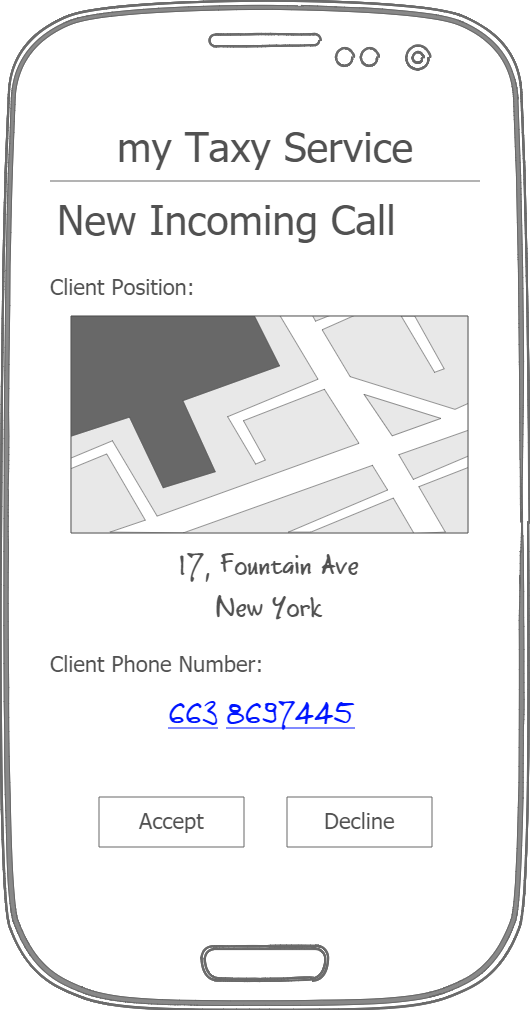
\includegraphics[height=.8\textheight]{Mockup-TaxiDriversNewIncomingCall}
		\centering
  \end{column}
  \begin{column}{.5\textwidth}
    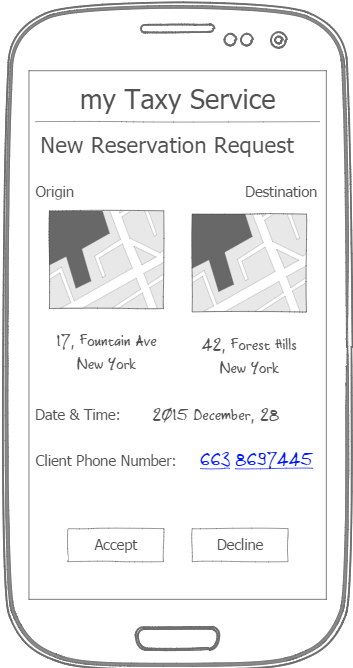
\includegraphics[height=.8\textheight]{Mockup-TaxiDriversReservationRequest}
		\centering
  \end{column}
\end{columns}
\end{frame}

\subsection {The World and The Machine}

\begin{frame}{\currentname}

\begin{figure}[H]
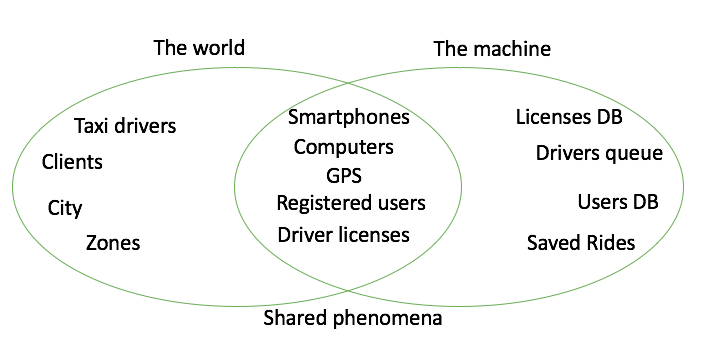
\includegraphics[width=.9\textwidth]{WorldAndMachine}
\centering
\end{figure}

\end{frame}

\subsection{Use Cases}

\begin{frame}{\currentname}

\framesubtitle{Client}

\begin{figure}[H]
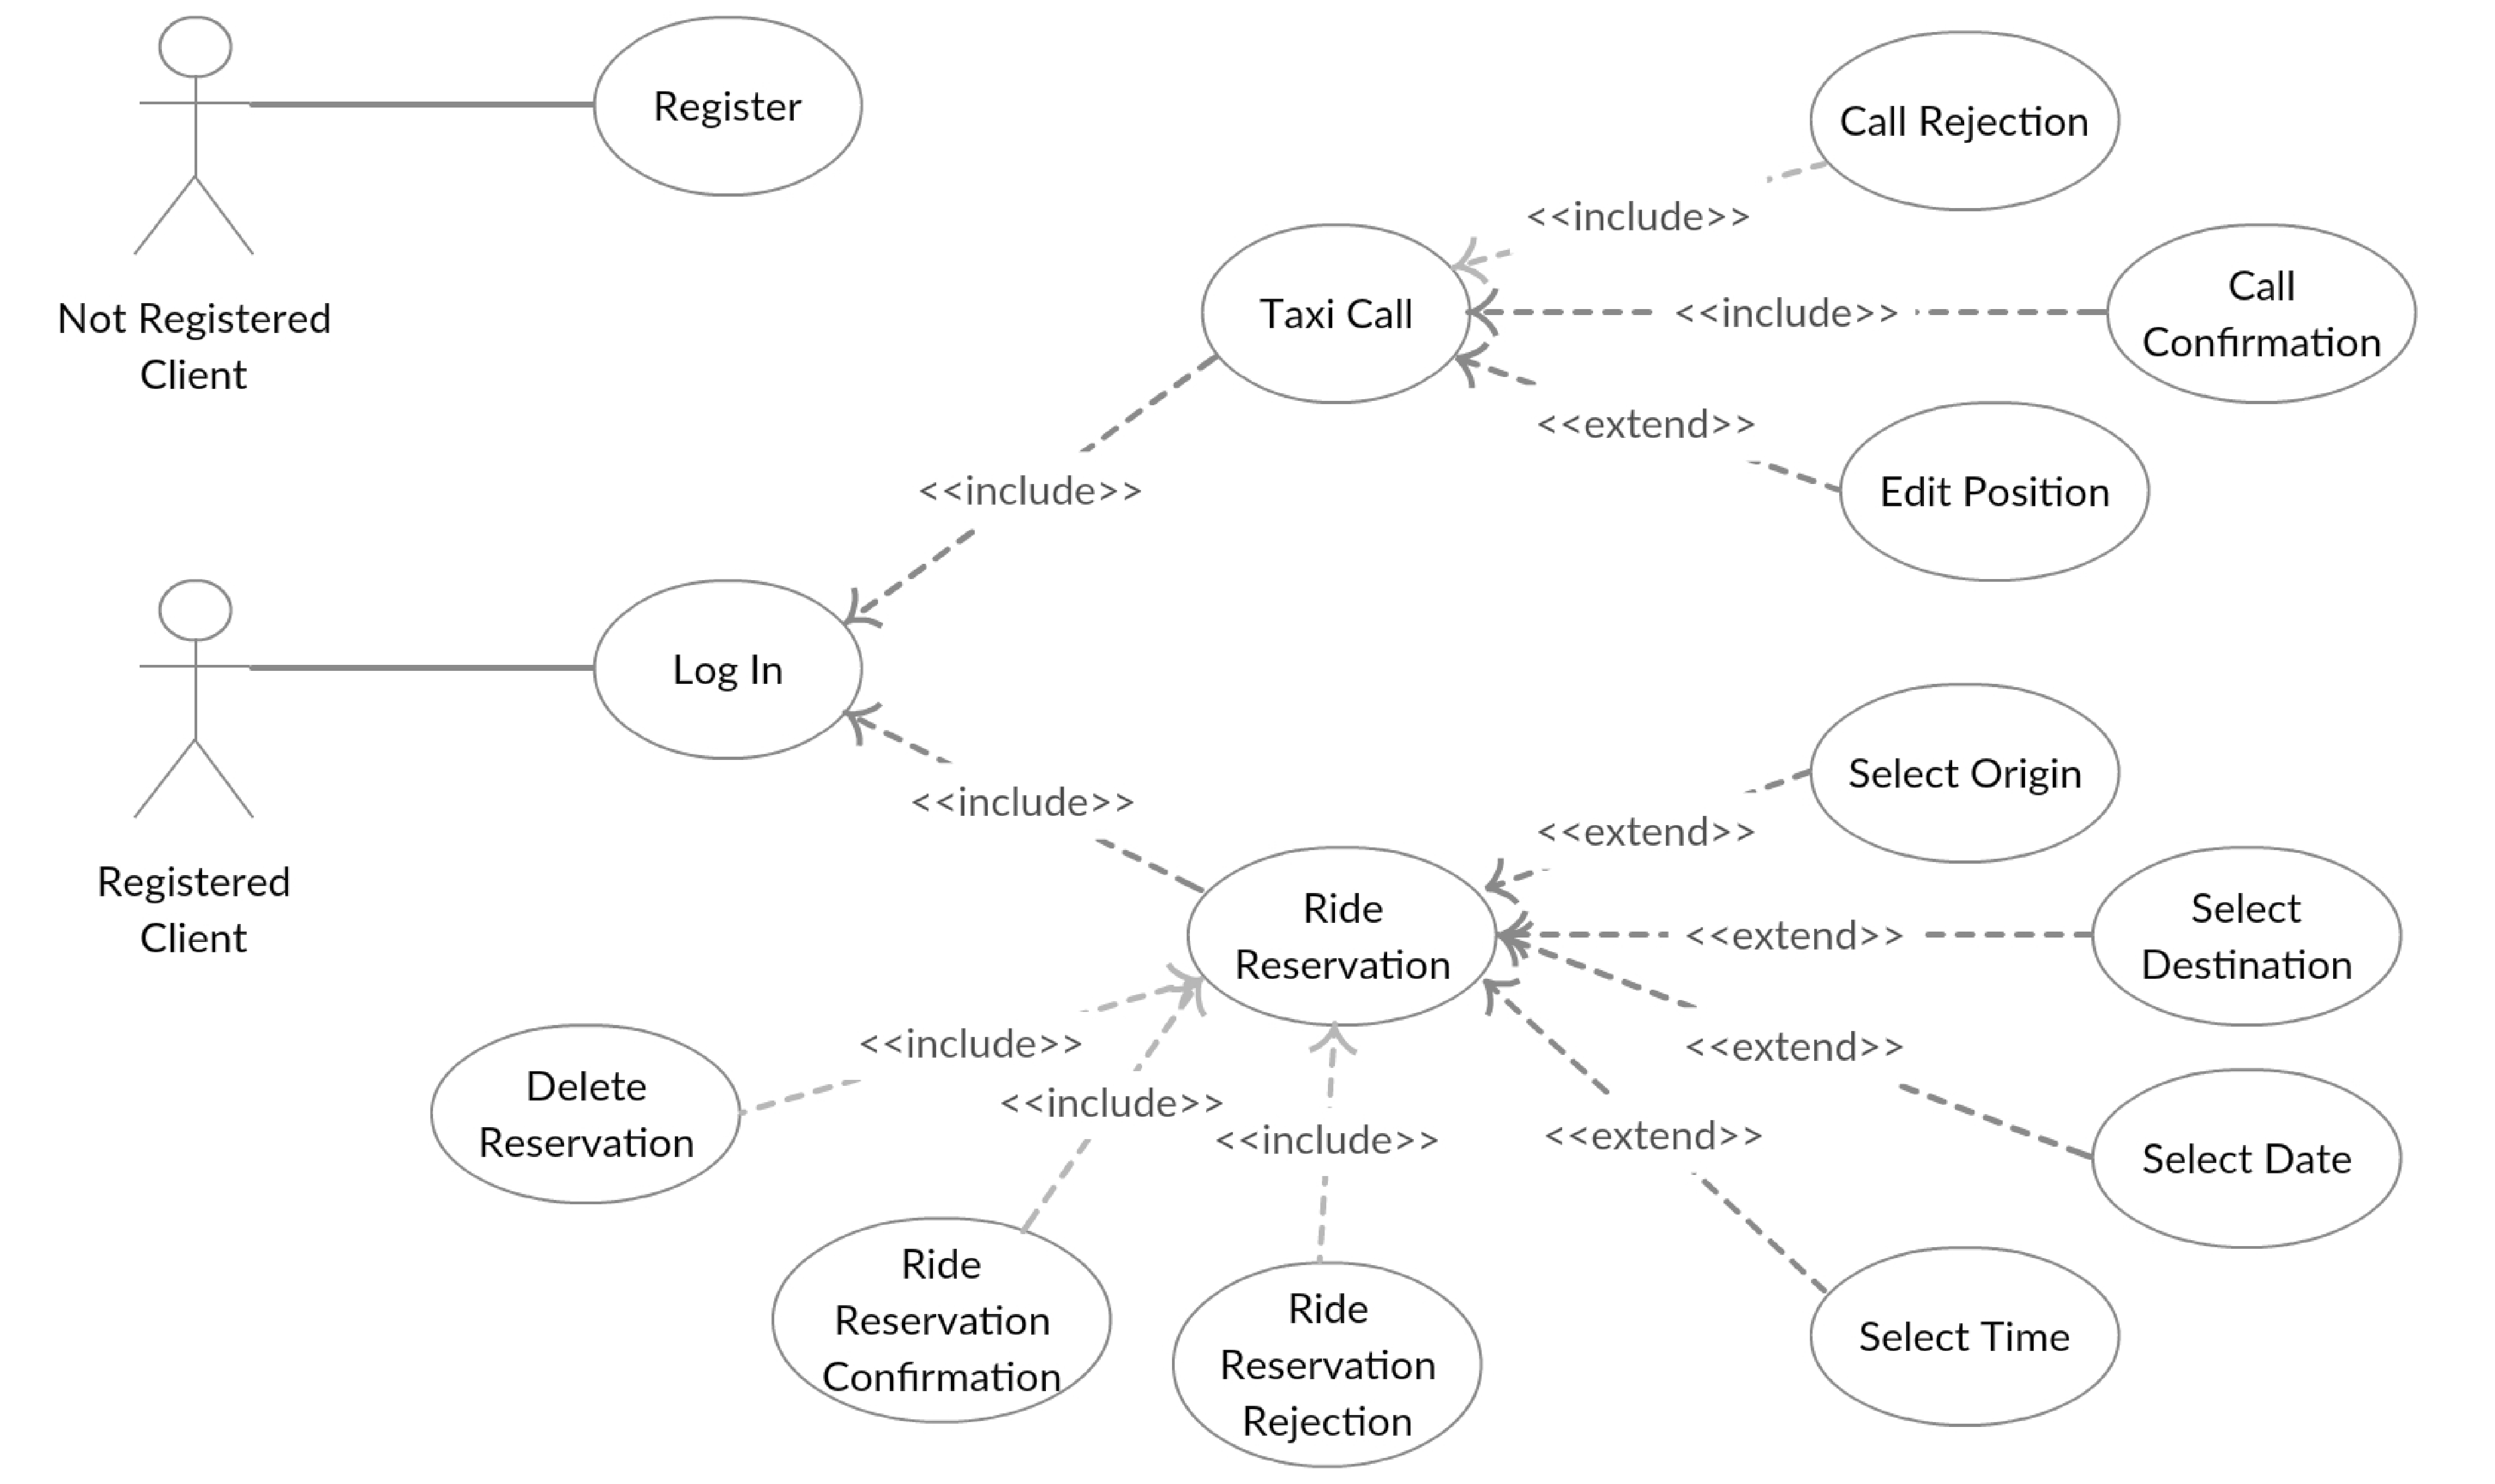
\includegraphics[width=.9\textwidth]{UseCase-Client}
\centering
\end{figure}

\end{frame}

\begin{frame}{\currentname}

\framesubtitle{Taxi Driver}

\begin{figure}[H]
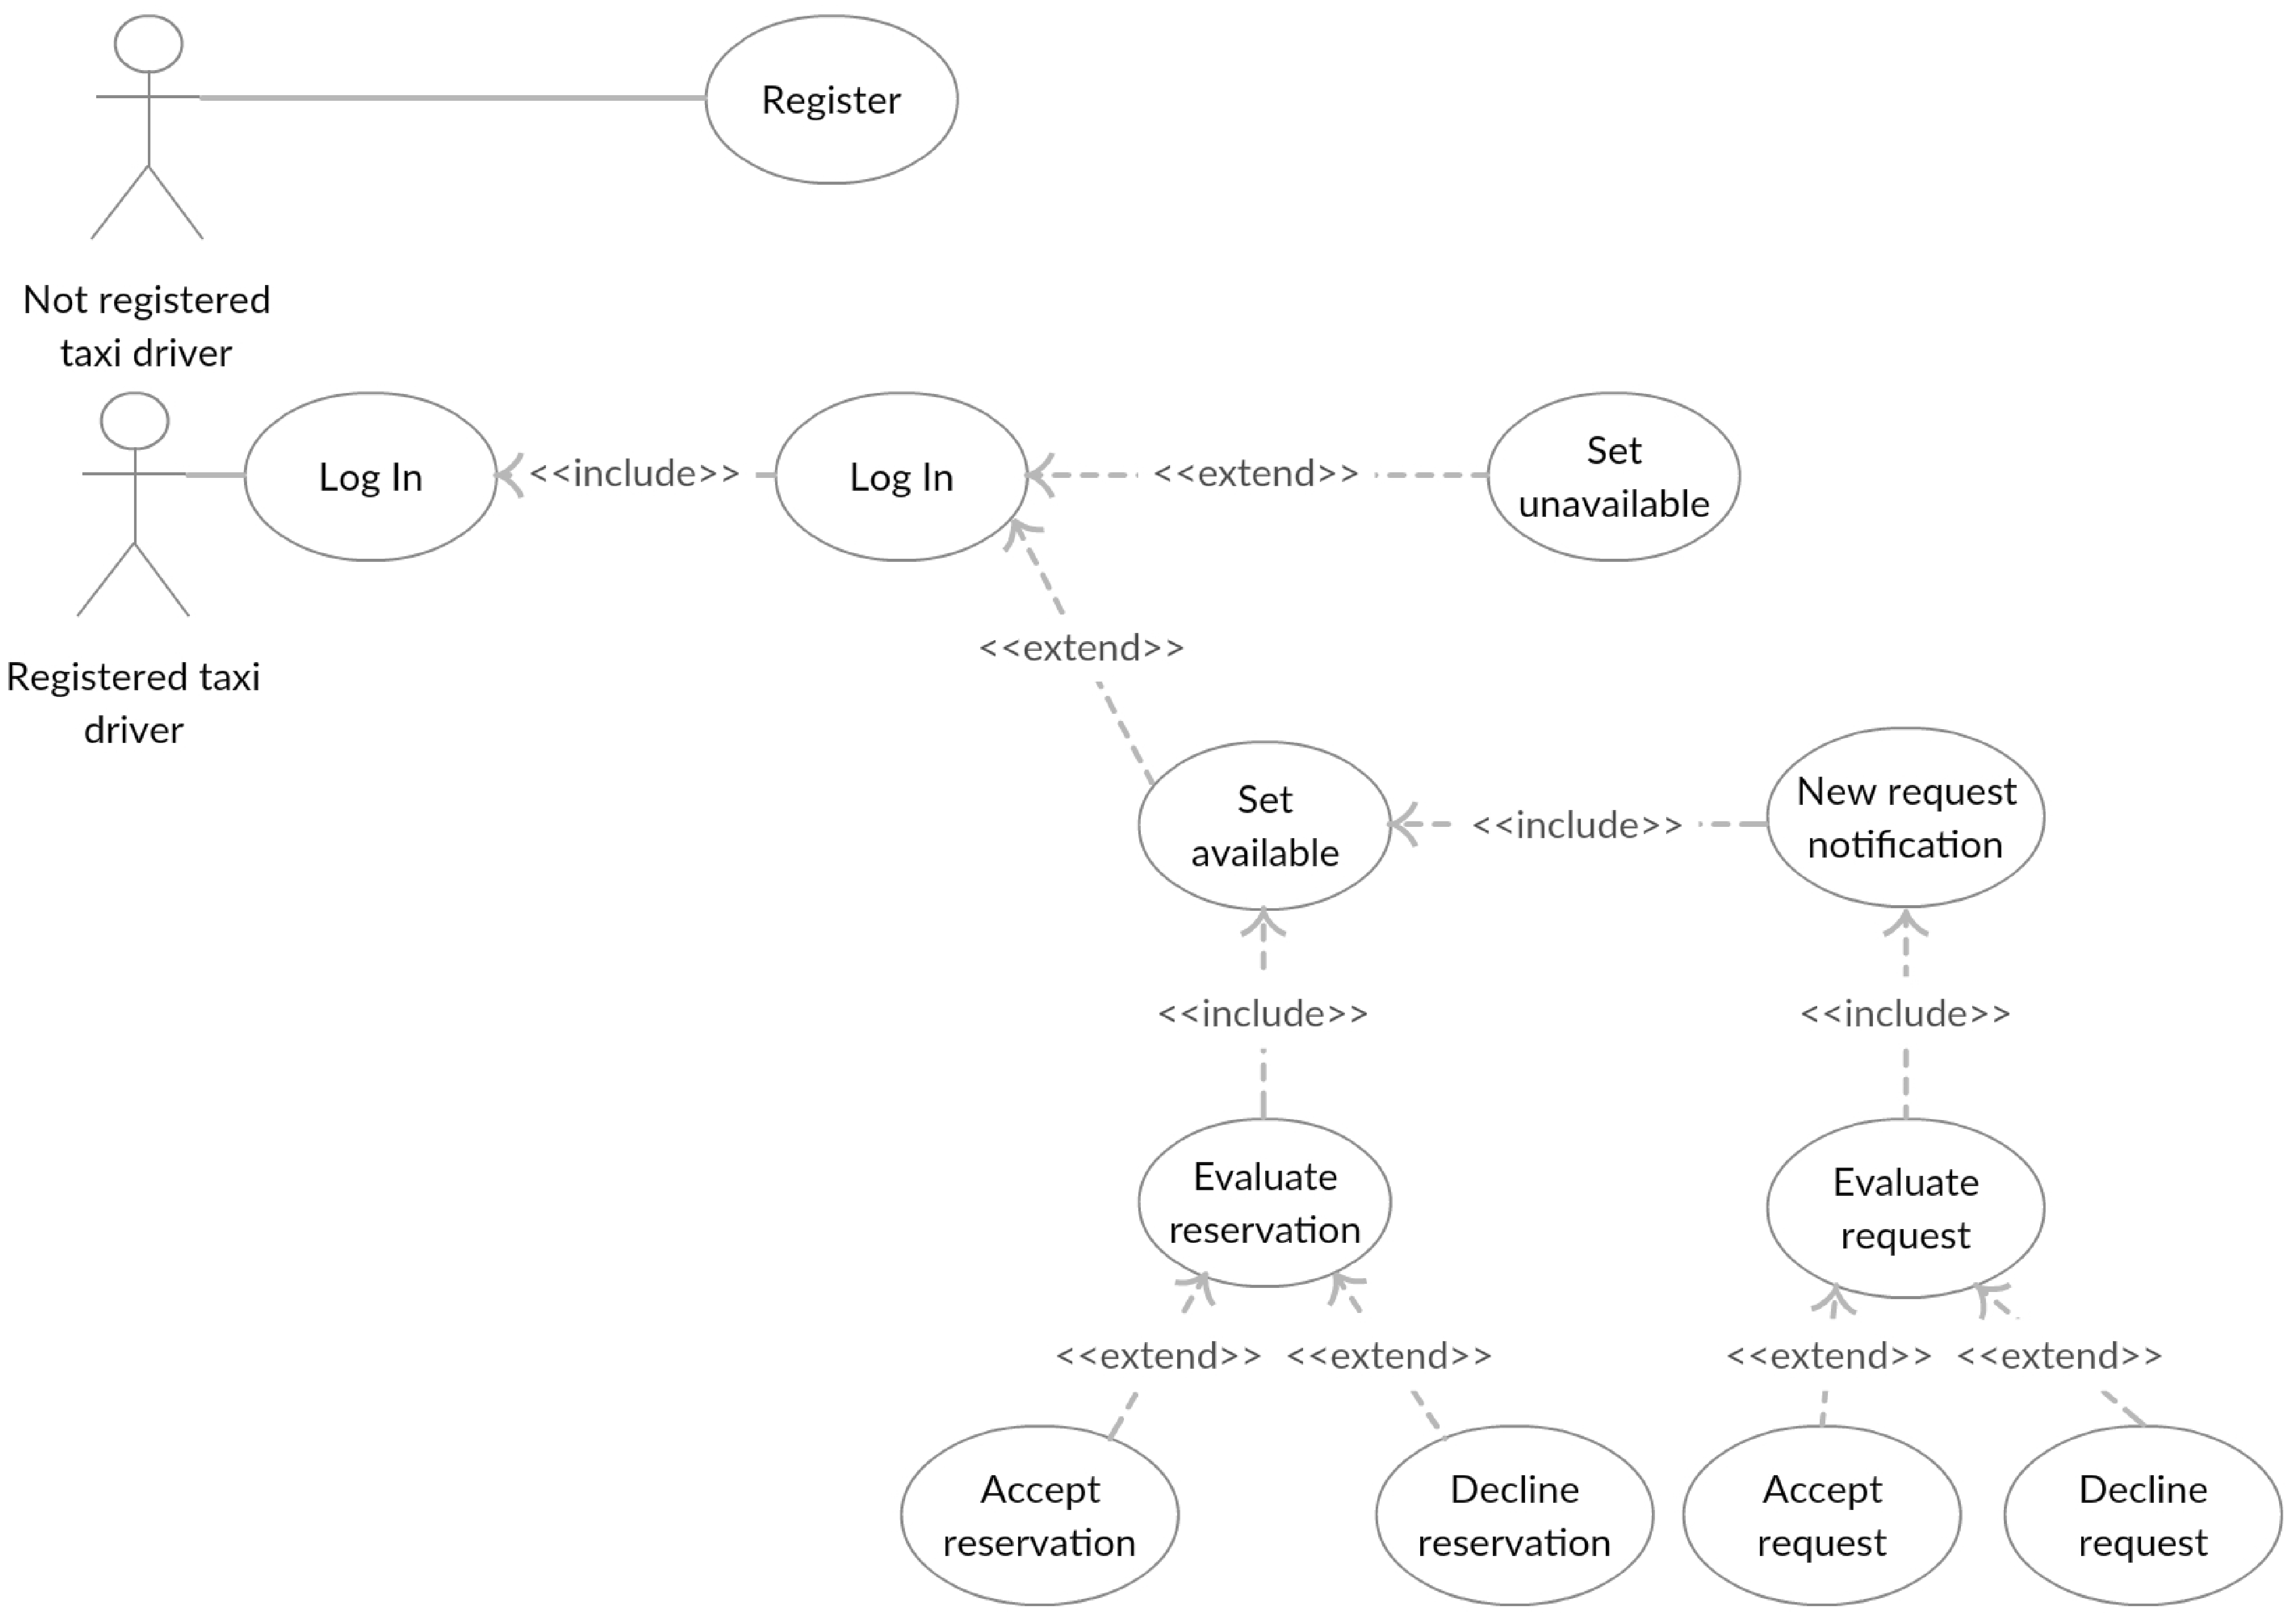
\includegraphics[width=.9\textwidth]{UseCase-TaxiDriver}
\centering
\end{figure}

\end{frame}

\subsection {Alloy}

\begin{frame}{\currentname}

\begin{figure}[H]
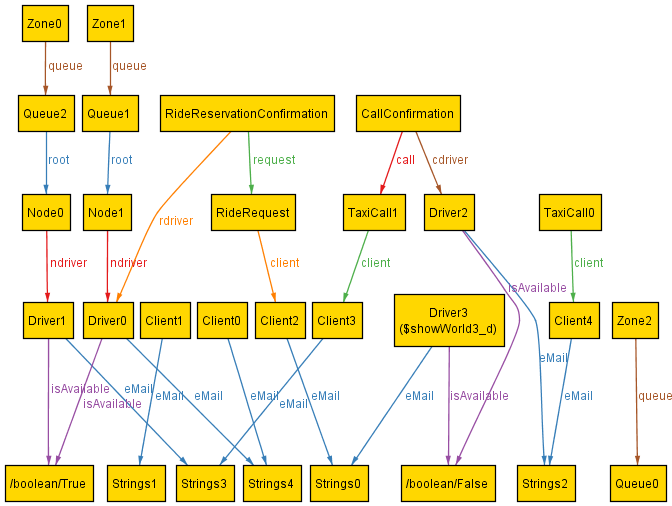
\includegraphics[height=.8\textheight]{Alloy-FreeDriver}
\centering
\end{figure}

\end{frame}